In this section, we describe a different strategy that aims to avoid the following too restrictive behavior: the strategy used in \cite{Mitsch-RSS-13} only reason about distance to the obstacle. This means that a straight line trajectory should keep a uselessly large distance to obstacles on the side (see Figure~\ref{OA}).

Again, we consider a moving vehicle and we add an interaction with an operator. The operator would like to move the vehicle by giving driving directions, that is, a desired instantaneous speed, and these directions must be rejected if they make the vehicle run into the obstacle.
This is because the operator may not have paid attention, or because the communication link may be compromised by an attacker.

\begin{figure}[ht]
\begin{center}
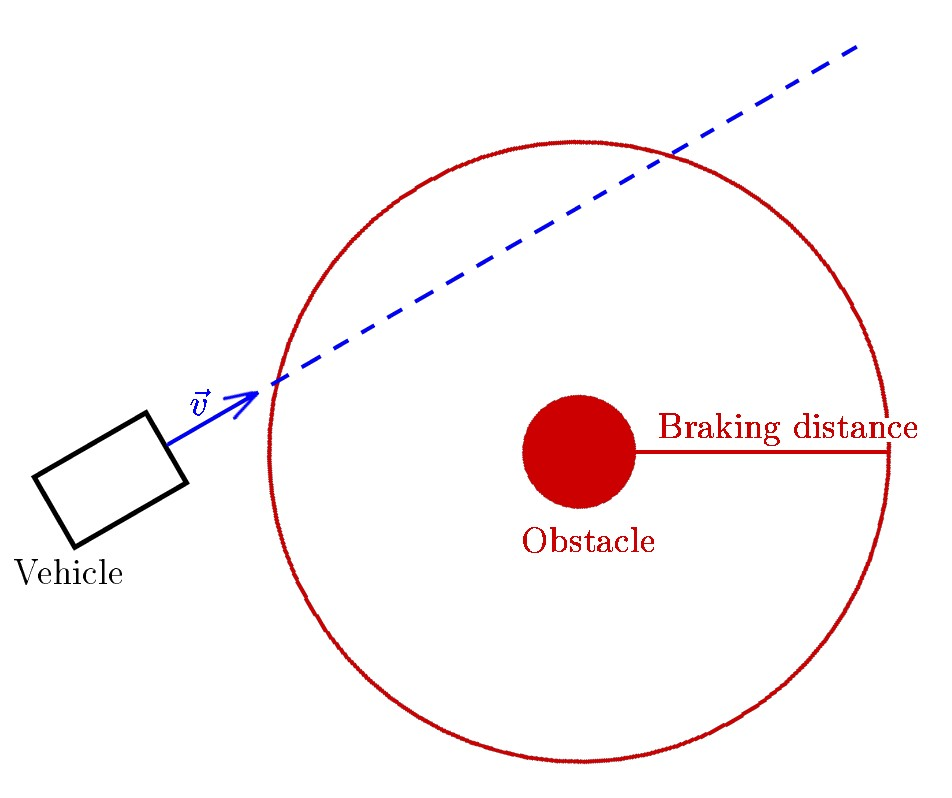
\includegraphics[height=8cm]{trajectory.jpg}
\caption{A safe but unacceptable trajectory}\label{OA}
\end{center}
\end{figure}

\subsection{Physical model and hypothesis}

We assume that the obstacle is fixed and given by its absolute position (GPS coordinates), and the vehicles sensors also give its absolute position.
Operator commands are given by an absolute speed (direction and velocity) to set to the vehicle, which should be either accepted or causing the vehicle to stop to stay at a minimal safe distance $D$ of the obstacle.
If the vehicle is already below this safe distance, we should only accept command that take the vehicle away from the obstacle.

The system could be represented as follows: A sensor node communicates the position to the controller through a $\mathit{Input}$ topic, and the controller node sends commands to the engine to set the new speed with the $Output$ topic. 
The controller node is also responsible for the communication with the operator. %(see Figure \ref{...})
For more simplicity, we model this link by a variable \texttt{OpCommand}, accessible by the controller and supposed to be updated each time a new command is received from the operator.

% Add beautiful schema here

We assume there is a known function $b(v)$ that, for a velocity $v$, gives the distance used to stop completely from the moment the vehicle begins to brake\footnote{$ $
In case the vehicle purposely doesn't brake at full power when the speed is too high to avoid tilting}.
In other cases, we assume that the new speed is set immediately after the command is computed by the engine node (in usual conditions, commands given by an operator -- that are not "stop!" -- are small variations of the current speed).
This would only add complexity to the explanations, but not change fundamentally the ideas presented here, so we assume the position is known exactly, and that the speed after a computation of the engine is exactly the speed contained in the received command.
Finally, we assume the parameters of the $Output$ topic are chosen in such a way that the message order is preserved.

\subsection{Controller strategy}

We use the same notations as in section~\ref{MAdef}, except for the engine node noted $E$ and its execution noted $e(n)$.
Because the system is asynchronous, when the controller receives a position from the sensor, the actual position may have changed depending on previous set speeds.
We also need to consider the potential delay before a command issued by the controller is executed by the engine.

We assume the controller keeps a buffer of the $N$ previous set speeds with
\[N = \left\lceil \frac{MA(Input) + MA(Output) + maxT(E)}{minT(C)} \right\rceil\]
Initially, this buffer is filled with zeros and each time a command is sent, the corresponding speed is added at the end of the buffer (after removing the first value).

This way, the buffer contains at time $t$ all speeds that were sent from $t - \big ( MA(Input) + MA(Output) + maxT(E) \big )$ to $t$. So, assume the controller executes $c(n)$ and $s(k)$ is the sensor message that is used, then for all time $t$ in $[s(k), c(n)]$, the actual speed at time $t$ is contained in the buffer.
We assumed $Output$ preserves the message order, so for $t$ in $[c(n), e(l)]$ (where $e(l)$ is a step of the engine that uses $c(n)$), the actual speed at time $t$ is in the updated buffer.

\paragraph{ }For each speed $\vec{v} = v.\vec{u}$ in the buffer and in the variable \texttt{OpCommand}, we compute the set of positions $Unsafe(\vec{v})$ that are at a distance less than $b(v)$ in the direction $\vec{u}$ from the unsafe zone\footnote{i.e. the points at a distance less than $D$ to the obstacle, assumed to be the origin}:
\[Unsafe(\vec{v}) = \Big \{ P \,| \, \exists d \leq b(v), \, \| P + d.\vec{u} \| \leq D \Big \} \]

Then, we extend this zone considering the buffered speeds and the new desired speed. More precisely, we consider the positions from which we can get in $Unsafe(\vec{v})$ using some composition of these speeds in less than $\lambda = MA(Input) + MA(Output) + maxT(E)$. 
Formally, let \mbox{$(\vec{v_1}, \dots, \vec{v_n})$} be the buffer, and $\vec{v_0}$ the speed contained in \texttt{OpCommand}. Then, the extended zone is:
\[Unsafe_{ext}(\vec{v}) = \left\{ P \,| \quad
\exists t_0, \dots, t_n, \quad \sum_{i=0}^N t_i \leq \lambda \, \textrm{ and } \,
P + \sum_{i=0}^N t_i.\vec{v_i} \in Unsafe(\vec{v}) \right\} \]

If the measured position is inside one of the $Unsafe_{ext}(\vec{v_i})$, the vehicle should stop, so the controller sends a command containing a zero speed. Otherwise, it is safe to proceed the user's instruction.
In both cases, the buffer must be actualized.


\subsection{Elements of correctness proof}

The main argument is quite simple: the vehicle runs into the obstacle if it doesn't brake soon enough, that is, at some point, the vehicle has a speed $\vec{v}$, is in $Unsafe(\vec{v})$ and is not braking.
With said strategy, this is not possible.

Assume at time $T$, the vehicle is in this situation. The speed was set during a computation $e(n)$ of the engine according to a command $c(k)$ from the controller.
When $c(k)$ occurred, we had $\texttt{OpCommand} = \vec{v}$ ($\vec{v} \neq \vec{0}$ is the command that was sent), and let $B$ be the state of the buffer at this point (before update).
The controller made the decision to send the command $\vec{v}$ according to this speed, the buffer state $B$, and a position measured at $s(l)$; and (among others) $s(l) \notin Unsafe_{ext}(\vec{v})$ -- otherwise the controller would have sent the stop order.

We know by definition of the buffer that for $t \in [s(l), c(k)]$, the speed at time $t$ was in $B$,
and for $t \in [c(k), e(n)]$, the speed at time $t$ was in the updated buffer. Also, for $t \in [e(n), T]$, the speed was $\vec{v}$. 
In each case, the speed was in $B \bigcup \{ \vec{v} \}$.
By definition of these bounds, we have $T - e(n) \leq maxT(E)$, $e(n) - c(k) \leq MA(Output)$ and $c(k) - s(l) \leq MA(Input)$.
This means the vehicle went from outside $Unsafe_{ext}(\vec{v})$ to inside $Unsafe(\vec{v})$ in less than $\lambda$, which is impossible by assumption.


\subsection{Future work}

Unlike properties given in Sections 4 to 6, this result has not been formally proved with PVS, so such an implementation is a first possible extension.
However, the proof needs first to be completed before being mechanically verified: an identified gap is the influence of zero speeds added to the buffer when the \emph{stop} command is sent.
Actually, the assumption is that for all $t$ in some past time interval, the speed at time $t$ is in the buffer, but (unlike non-zero speeds) when a zero speed is processed by the engine, the speed is not set to 0 immediately because of the braking distance.
This could be solved by more assumptions on the engine node; for example, when the \emph{stop} command is processed, all other commands are ignored until the vehicle has come to full stop, plus some delay to cover communication latency.

Also, it could be helpful to find linear approximations of used sets (especially $Unsafe_{ext}(\vec{v})$) in order to reduce computing time. 
Another direction could be to replace the speed buffer by a measured value and dynamic properties of the vehicle (acceleration power / direction change capabilities).
This would give a more realistic physical model, but it would need a more complex analysis to ensures the vehicle responds to operator commands.







